%\documentclass[aps,prd,nofootinbib]{revtex4-1}
\documentclass[singlepage,notitlepage,nofootinbib,11pt]{revtex4-1}
\usepackage{amsmath}
\usepackage{graphicx}
\usepackage{subfig}
\usepackage{epsfig}
\usepackage{listings}
\usepackage[hidelinks,hyperfootnotes=false,bookmarks=false,colorlinks=true]{hyperref}

\newcommand{\eq}[1]{\begin{align*}#1\end{align*}}
\newcommand{\pmat}[1]{\begin{pmatrix}#1\end{pmatrix}}
\newcommand{\center}[1]{\begin{center}#1\end{center}}
\def\<{\langle}
\def\>{\rangle}
\def\l{\left}
\def\r{\right}


\begin{document}
\title{Problem Set 5 - G6080}
\author{Victor Genty}
\email{vgenty@nevis.columbia.edu}
\homepage{www.nevis.columbia.edu/~vgenty}
\date{\today}
\begin{abstract}
\centering
Source code can be found at \href{https://github.com/vgenty/G6080/tree/master/ps5}{github.com/vgenty/G6080/ps5}
\end{abstract}
\maketitle
\section{Poisson's Equations}


\begin{figure}[h]
  \centering
  \captionsetup[subfigure]{labelformat=empty}
  \subfloat[][]{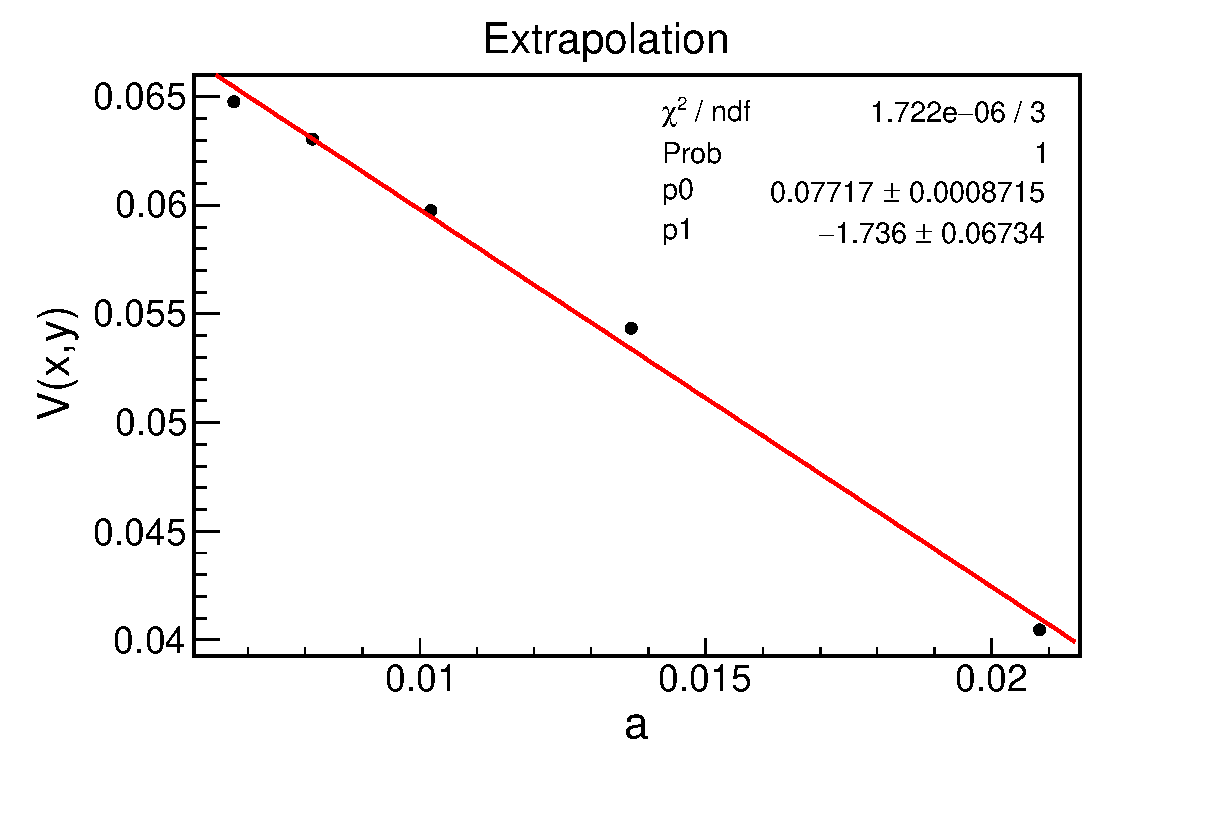
\includegraphics[width=0.5\textwidth]{figures/ex1.eps}}
  \subfloat[][]{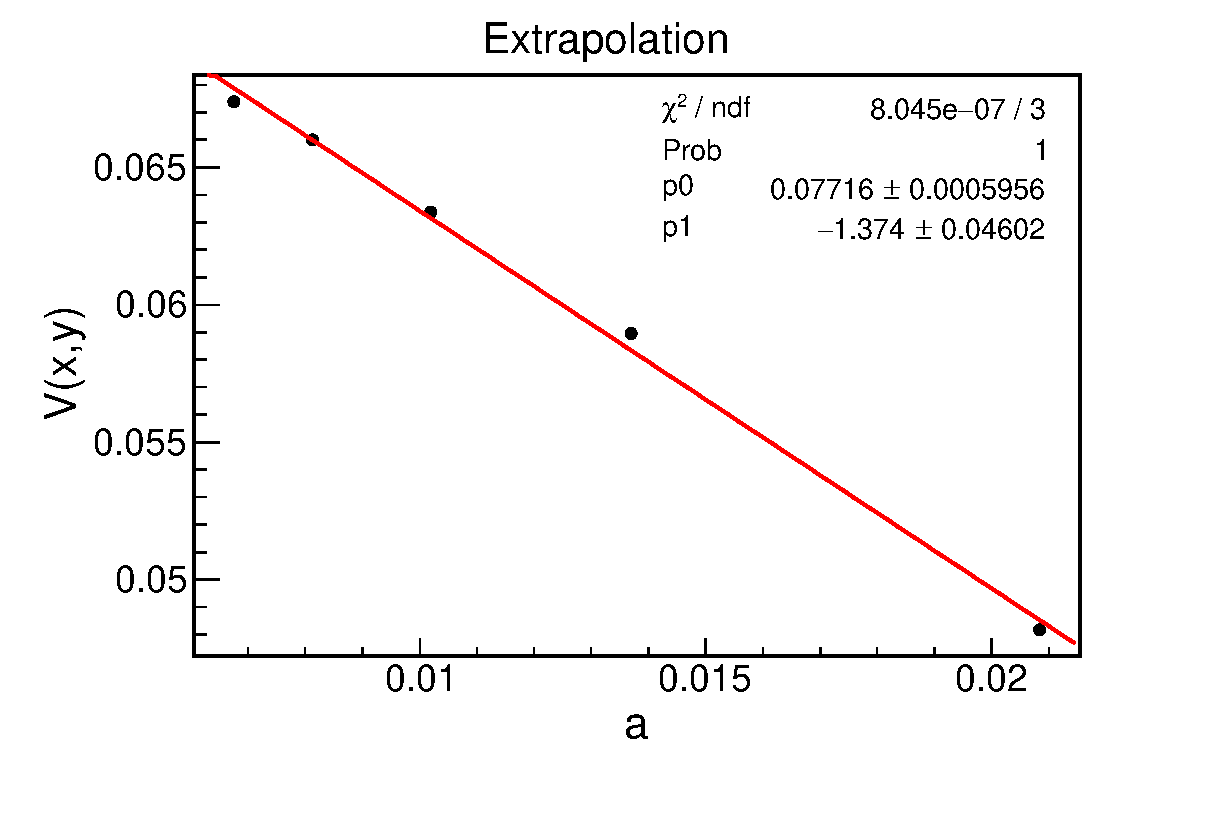
\includegraphics[width=0.5\textwidth]{figures/ex2.eps}}
  \caption{\label{extrapolation} Extrapolation of the grid spacing to zero $a$ for two nearby points on the the 2D grid. The fit parameters are shown in the top right of each plot. The variable p0 shows the y-intercept and $a=0$ extrapolation.}
\end{figure}

\begin{figure}[h]
  \centering
  \captionsetup[subfigure]{labelformat=empty}
  \subfloat[][]{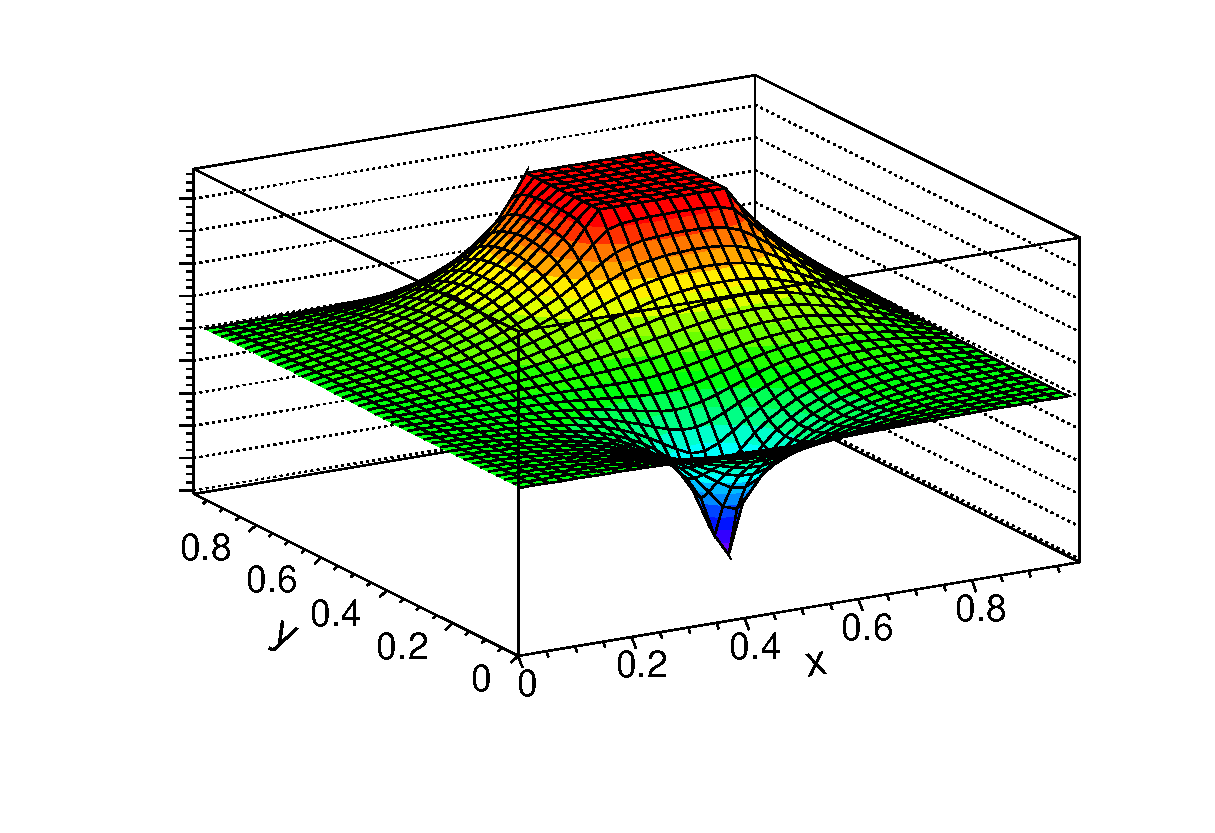
\includegraphics[width=0.5\textwidth]{figures/poisson.eps}}
  \subfloat[][]{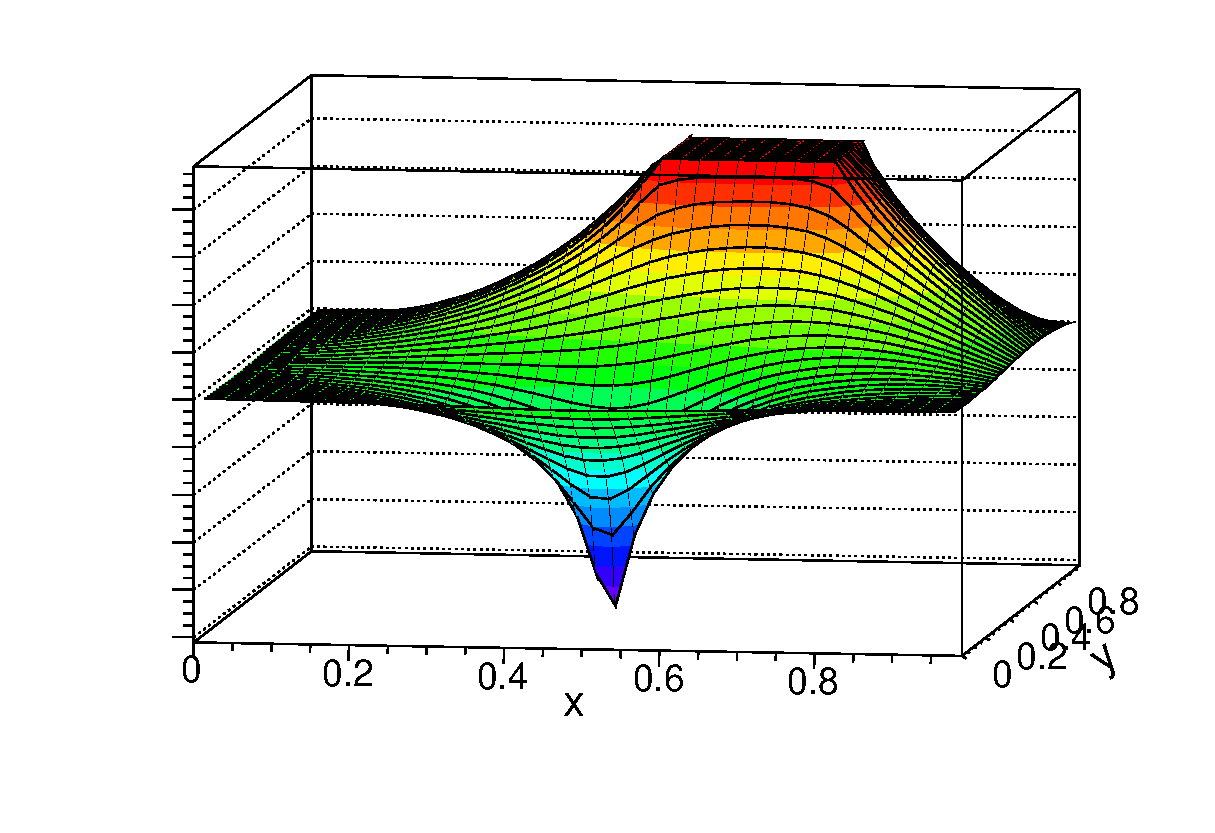
\includegraphics[width=0.5\textwidth]{figures/poisson2.eps}}\\
  \subfloat[][]{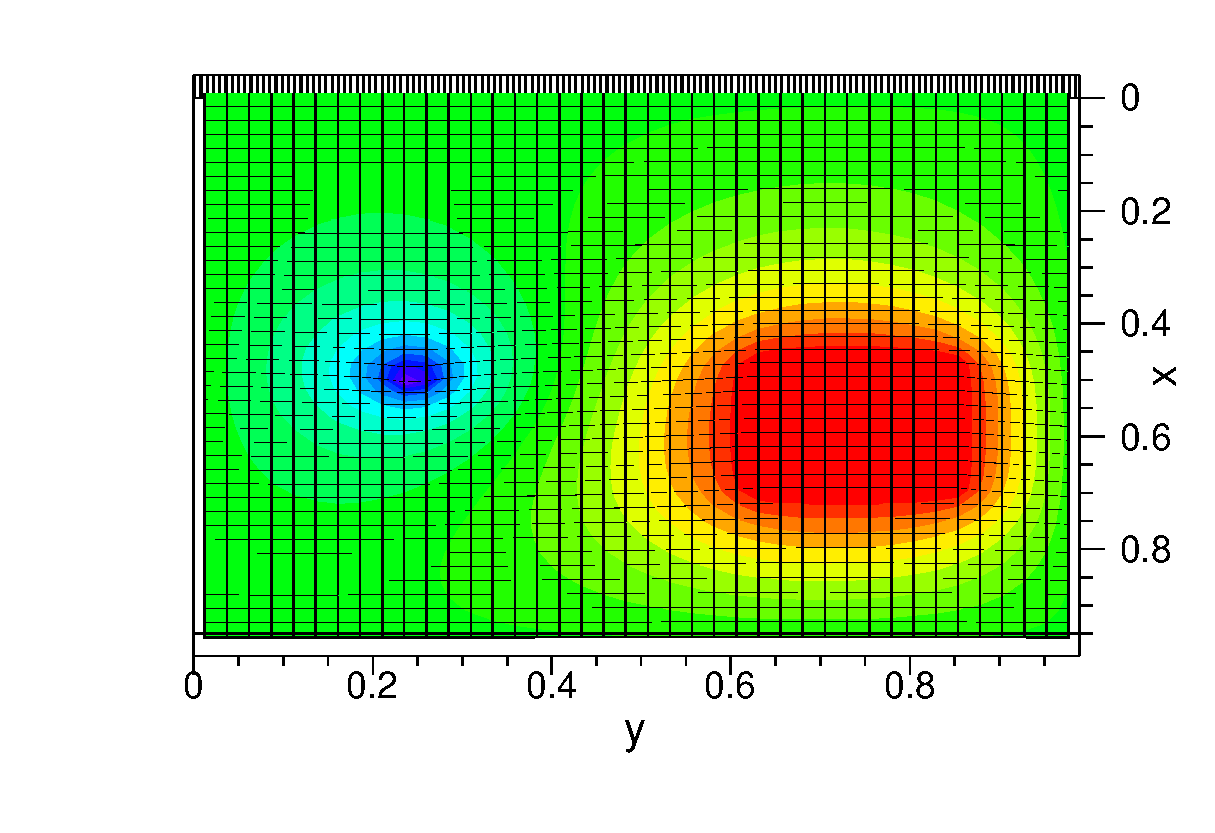
\includegraphics[width=0.5\textwidth]{figures/poisson3.eps}}
  \subfloat[][]{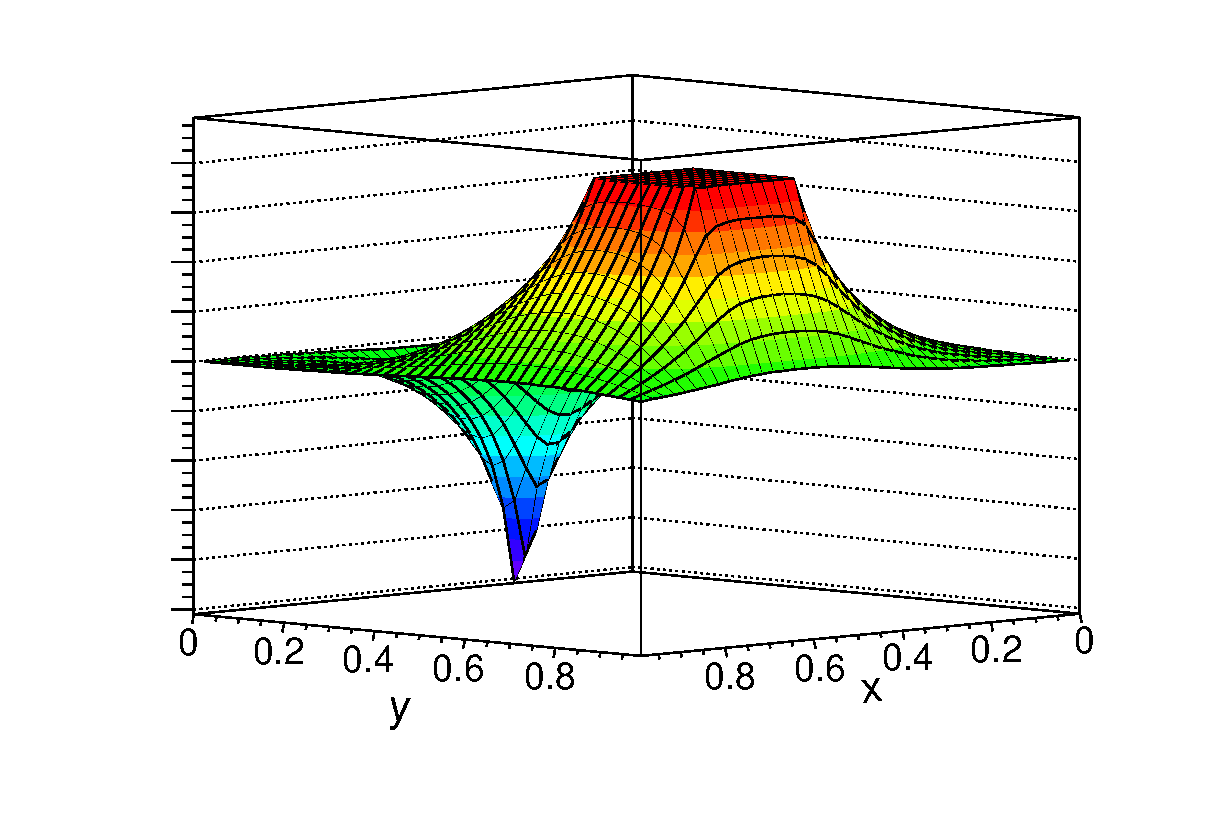
\includegraphics[width=0.5\textwidth]{figures/poisson4.eps}}
  \caption{\label{poissons} ``SURF'' plot for 2D discrete poisson solver with grid size $a\sim0.01$. The deep blue color is most negative, red being the largest, and green representing zero.}
\end{figure}

\clearpage
\section{Free particle Schrodinger equation}


\clearpage
\section{Charged particle Schrodinger equation}


\end{document}
